% --- ETUDE DE CAS ---
\newpage
\section*{Étude de cas~: Docker}
\addcontentsline{toc}{section}{Étude de cas~: Docker}

\section*{AAV}
\addcontentsline{toc}{section}{AAV}
\begin{itemize}
	\item [2] Connaître / comprendre le mécanisme de communication des sockets
	\item [2] Connaître / comprendre le principe de fonctionnement de l'architecture Client-Serveur
	\item [5] Transmission de flux
	\item [5] Développer une IHM Client-Serveur manipulant des sockets en C\#
\end{itemize}

\newpage

\subsection*{Mots clés}
\phantomsection
\addcontentsline{toc}{subsection}{Mots clés}
\begin{itemize}
	\item Conteneur Docker
	\item Unité de traitement
	\item Ports IP
	\item Architecture client-serveur
	\item Socket
	\item Flux de données
\end{itemize}

\subsection*{Contexte}
\phantomsection
\addcontentsline{toc}{subsection}{Contexte}
\noindent Le client souhaite avoir une vision sur l'état d'avancement de la fabrication de ses chaînes de production. 

\subsection*{Problématique}
\phantomsection
\addcontentsline{toc}{subsection}{Problématique}
\noindent Comment envoyer les données à distance au client et héberger l'application de visualisation ?

\subsection*{Contraintes}
\phantomsection
\addcontentsline{toc}{subsection}{Contraintes}
\begin{itemize}
	\item Serveur Docker en DMZ
	\item Code fourni
\end{itemize}

\subsection*{Généralisation}
\phantomsection
\addcontentsline{toc}{subsection}{Généralisation}
\begin{itemize}
	\item Socket C\#
	\item Conteneurisation
	\item IPC
\end{itemize}

\subsection*{Livrables}
\phantomsection
\addcontentsline{toc}{subsection}{Livrables}
\begin{itemize}
	\item Code complet
	\item Plan d'utilisation Docker
\end{itemize}

\subsection*{Pistes de solutions}
\phantomsection
\addcontentsline{toc}{subsection}{Pistes de solutions}
\begin{itemize}
	\item Utiliser une architecture client-serveur avec des sockets pour envoyer les données à distance
	\item Conteneuriser l'application de visualisation avec Docker pour faciliter son déploiement et son hébergement
	\item Mettre en place une communication sécurisée entre le serveur Docker en DMZ et le client pour protéger les données transmises
\end{itemize}

\subsection*{Plan d'actions}
\phantomsection
\addcontentsline{toc}{subsection}{Plan d'actions}
\begin{itemize}
    \item Étudier les concepts de conteneurisation avec Docker et les mécanismes de communication avec les sockets
    \item Étudier les différentes options de communication sécurisée pour protéger les données transmises entre le serveur Docker et le client
    \item Étudier le fonctionnement de Socket et comment l'utiliser pour envoyer des données à distance en C\#
	\item Étudier le code fourni pour comprendre les données à transmettre et les besoins de l'application de visualisation
	\item Configurer un serveur Docker en DMZ pour héberger l'application de visualisation
	\item Conteneuriser l'application de visualisation avec Docker
	\item Mettre en place la communication sécurisée entre le serveur Docker et le client pour envoyer les données à distance
	\item 
\end{itemize}

\newpage
\section*{Démarche~: Docker}
\addcontentsline{toc}{section}{Démarche~: Docker}


\subsection*{Définition~: Mots clés}
\phantomsection
\addcontentsline{toc}{subsection}{Définition: Mots clés}

\noindent \textbf{Conteneur Docker}:
\noindent Un conteneur Docker est une unité de traitement légère et portable qui encapsule une application et toutes ses dépendances, permettant ainsi de garantir que l'application fonctionne de manière cohérente dans différents environnements.

\begin{center}
\rule{5cm}{0.4pt}
\end{center}

\vspace{0.5cm}

\noindent \textbf{Unité de traitement}:
\noindent Une unité de traitement est une ressource informatique qui peut exécuter des tâches ou des processus. Dans le contexte de Docker, un conteneur est considéré comme une unité de traitement car il peut exécuter une application de manière isolée.

\begin{center}
\rule{5cm}{0.4pt}
\end{center}

\vspace{0.5cm}

\noindent \textbf{Architecture client-serveur}:
\noindent Une architecture client-serveur représente l'environ-nement dans lequel des applications de machines clientes communiquent avec des applications de machines de type serveurs.

\vspace{0.5cm}

\noindent L’exemple classique est le navigateur Web d’un client qui demande (on parle de “requête”) le contenu d’une page Web à un serveur Web qui lui renvoie le résultat (on parle de “réponse”).
\begin{center}
	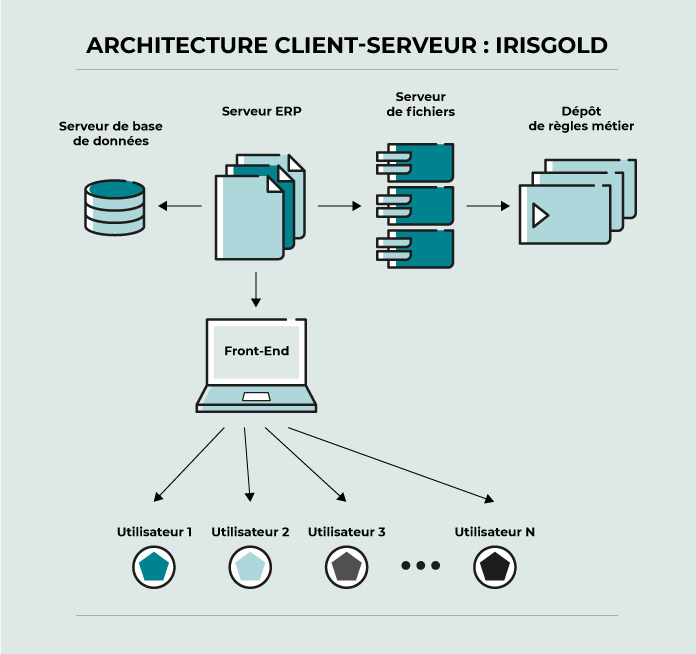
\includegraphics[width=0.6\textwidth]{contents/img/client-server.png}
\end{center}

\newpage

\noindent \textbf{Socket}:
\noindent Un socket est un point de communication utilisé pour établir une connexion entre deux processus sur un réseau. 

\vspace{0.5cm}

\begin{center}
\begin{tabular}{|p{0.25\textwidth}|p{0.65\textwidth}|}
\hline
\textbf{Méthode} & \textbf{Description} \\ \hline
\texttt{Socket.Bind} & Lie la socket à un point de communication, renvoie une erreur si le port spécifié par le point de communication est déjà utilisé par un autre processus \\ \hline
\texttt{Socket.Listen} & Place en file d'attente (queue) toutes les connexions entrantes \\ \hline
\texttt{Socket.Accept} & Lit la file d'attente et accepte les connexions entrantes. Accept est bloquant, l'exécution du code est bloquée jusqu'à ce qu'accept détecte une connexion entrante dans la file d'attente \\ \hline
\texttt{Socket.Select} & Permet entre autres de vérifier si une socket connectée tente d'écrire quelque chose. En passant un tableau de connexion en paramètre à select, après l'exécution de select, le tableau ne contient plus que les sockets ayant des données prêtes à être lues \\ \hline
\texttt{Socket.Poll} & Permet, un peu comme select, de détecter si une socket est prête à être lue ou écrite. À l'inverse de select, elle permet aussi de détecter si une connexion est terminée \\ \hline
\texttt{Socket.Receive} & Permet de réceptionner les données qui ont été écrites sur la socket \\ \hline
\texttt{Socket.Send} & Permet d'écrire des données sur une socket \\ \hline
\texttt{Socket.Connect} & Permet de se connecter à une socket \\ \hline
\end{tabular}
\end{center}

\vspace{0.5cm}

\noindent \textbf{Important}: Manipuler des sockets bruts demande de bien gérer l'asynchronisme (Task, async/await) pour éviter de bloquer votre application pendant que vous attendez une réponse du réseau.

\begin{center}
\rule{5cm}{0.4pt}
\end{center}

\vspace{0.5cm}
\noindent \textbf{Flux de données}:
\noindent Un flux de données est une séquence de données qui est transmise d'un point à un autre. Dans le contexte de Docker, les flux de données sont utilisés pour envoyer des informations entre les conteneurs et les applications externes.

\begin{center}
\rule{5cm}{0.4pt}
\end{center}

\vspace{0.5cm}

\noindent \textbf{Ports IP}:
\noindent Un port IP est un point de communication utilisé pour identifier une appli-cation ou un service spécifique sur un réseau. Dans le contexte de Docker, les ports IP sont utilisés pour permettre la communication entre les conteneurs et les applications externes.
    
\newpage

\section*{Corbeille check}
\addcontentsline{toc}{section}{Corbeille check}

\noindent \textbf{Question}: Compléter le code

\begin{minted}[tabsize=2]{csharp}
using System;
using System.Net;
using System.Net.Sockets;
using System.Text;

namespace Client {
	class Program {
		static void Main(string[] args) {

			IPHostEntry ipHost = Dns.GetHostEntry(Dns.GetHostName());
			IPAddress ipAddr = ipHost.AddressList[0];
			IPEndPoint localEndPoint = new IPEndPoint(ipAddr, 1200);

			Socket sender = new Socket(ipAddr.AddressFamily, SocketType.Stream,
			ProtocolType.Tcp);

			try {
				sender.Connect(localEndPoint);

				Console.WriteLine("Socket connecté à -> {0}");
				Console.WrtieLine(sender.RemoteEndPoint.ToString());

				byte[] messageSent = Encoding.ASCII.GetBytes("Test Client<EOF>");
				int byteSent = sender.Send(messageSent);
				byte[] messageReceived = new byte[1024];
				int byteRecv = sender.Receive(messageReceived);

				Console.WriteLine("Message du Serveur -> {0}",
					Encoding.ASCII.GetString(messageReceived, 0, byteRecv));

				sender.Shutdown(SocketShutdown.Both);
				sender.Close();

			} catch (ArgumentNullException ane) {
				Console.WriteLine("ArgumentNullException : {0}", ane.ToString());
			} catch (SocketException se) {
				Console.WriteLine("SocketException : {0}", se.ToString());
			} catch (Exception e) {
				Console.WriteLine("Unexpected exception : {0}", e.ToString());
			}
		}
	}
}
\end{minted}

\newpage

\noindent \textbf{Question}: Compléter le code

\begin{minted}[tabsize=2]{csharp}
using System;
using System.Net;
using System.Net.Sockets;
using System.Text;

namespace Server {
	class Program {
		static void Main(string[] args) {

			IPHostEntry ipHost = Dns.GetHostEntry(Dns.GetHostName());
			IPAddress ipAddr = ipHost.AddressList[0];
			IPEndPoint localEndPoint = new IPEndPoint(ipAddr, 11111);

			Socket listener = new Socket(ipAddr.AddressFamily, SocketType.Stream,
			ProtocolType.Tcp);

			try {
				listener.Bind(localEndPoint);
				listener.Listen(10);

				while (true) {
					Console.WriteLine("Waiting connection ... ");
					Socket clientSocket = listener.Accept();

					byte[] bytes = new Byte[1024];
					string data = null;

					while (true) {
						int numByte = clientSocket.Receive(bytes);
						data += Encoding.ASCII.GetString(bytes, 0, numByte);
						if (data.IndexOf("<EOF>") > -1)
							break;
					}
					Console.WriteLine("Text reçu -> {0} ", data);

					byte[] message = Encoding.ASCII.GetBytes("Test Server");
					clientSocket.Send(message);

					clientSocket.Shutdown(SocketShutdown.Both);
					clientSocket.Close();
				}
			} catch (Exception e) {
				Console.WriteLine(e.ToString());
			}
		}
	}
}
\end{minted}

\section*{Workshop}
\addcontentsline{toc}{section}{Workshop}

\newpage

\section*{Analyse et résolution : Docker}
\addcontentsline{toc}{section}{Analyse et résolution : Docker}

\subsection*{Conclusion}
\phantomsection
\addcontentsline{toc}{subsection}{Conclusion}

\newpage

\section*{Capitalisation}
\addcontentsline{toc}{section}{Capitalisation}

\begin{center}
\setlength{\tabcolsep}{10pt}

\begin{tabular}{|p{0.30\textwidth}|p{0.45\textwidth}|m{0.08\textwidth}|}
\hline
\textbf{AAV} & \textbf{Commentaire} & \textbf{Statut} \\ \hline

Définir Thread, Multi-threading, Mécanismes d'IPC, Ressource critique / Section critique, inter-blocage &
Les définitions de Thread, Multi-threading, IPC, Ressource critique, Section critique et inter-blocage sont fournies avec des exemples et explications claires. &
{\color{green!60!black}Acquis} \\ \hline

Citer, Décrire et expliquer les principaux problèmes liés à la section critique &
Les problèmes comme l'interblocage, la famine, l'inversion de priorité sont identifiés, expliqués et illustrés avec des solutions proposées. &
{\color{green!60!black}Acquis} \\ \hline

Citer, Décrire et expliquer les principaux mécanismes d'IPC et les organiser en catégories &
Les mécanismes d'IPC (sémaphores, mutex, etc.) sont présentés, catégorisés et expliqués avec des cas d'utilisation. &
{\color{green!60!black}Acquis} \\ \hline

Implémenter les mécanismes de synchronisation en C\# &
Des exemples de code C\# illustrent l'utilisation de Thread, ThreadPool, lock, Semaphore, Mutex pour la synchronisation. &
{\color{green!60!black}Acquis} \\ \hline

\end{tabular}
\end{center}

\newpage

\section*{Ressources}
\addcontentsline{toc}{section}{Ressources}

\begin{itemize}
	\item 
\end{itemize}
